\documentclass[9pt]{beamer}

\beamertemplatenavigationsymbolsempty
\renewcommand\mathfamilydefault{cmr}

\usepackage{pajmath}
\usepackage{booktabs}
\usepackage{colortbl}

\usepackage{tikz}
\usetikzlibrary{positioning,shapes.misc,calc,backgrounds,scopes} 
\usetikzlibrary{datavisualization}
\usetikzlibrary{datavisualization.formats.functions}
\tikzset{boxed/.style={
  thick,
  draw=black,
  top color=white,
  text height=1.5ex,
  text depth=.25ex
}}


\newcommand\lo{$-1$}
\newcommand\hi{$\phan1$}
\newcommand\ze{$\phan0$}
\newcommand\Ze{$\phan\Vzero$}
\newcommand\pskip{\pause\bigskip}
\newcommand\lspace{\addtolength{\itemsep}{0.5\baselineskip}}
\newcommand\red[1]{{\color{red}#1}}

\title{Reinforcement Learning:\\Value Functions}
\author{BIOE 498/598 PJ}
\date{Spring 2021}

\begin{document}
\frame{\titlepage}

\begin{frame}{Review}

\textbf{Last time}
\begin{itemize}\lspace
	\item RL agents learn by trial and error.
	\item RL problems are formulated as MDPs.
	\item Monte Carlo methods can find policies for RL problems.
	\item<2-> \textbf{Today:} How do random simulations lead to optimal policies?
\end{itemize}
	
\end{frame}

\begin{frame}{A Monte Carlo approach for Gridworld}

\begin{columns}
\begin{column}{0.5\textwidth}
	\begin{itemize}
		\item Each grid square is a state.
		\item Actions: move up, down, left, or right, but the agent cannot leave the grid.
		\item Reward: $-1$ for each step.
		\item Policy: Random.
	\end{itemize}
	
\bigskip
Starting from a random state, make random moves until the agent reaches the end.

\bigskip
Repeat may times and average the total rewards from each trajectory.

\bigskip
The policy is to move to squares with better Monte Carlo returns.
\end{column}

\begin{column}{0.5\textwidth}
	\begin{center}
		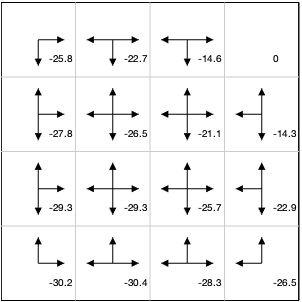
\includegraphics[width=\textwidth]{figures/gridworld1a.png}	
	\end{center}
\end{column}

\end{columns}

\end{frame}

\begin{frame}{Value functions}

\begin{itemize}\lspace
	\item We are using Monte Carlo to learn a \textbf{value function}.
	\item The value of a state is the expected reward from that state to the end of the trajectory:
		\[ V(s_i) = \mathbb{E}\left\{ \sum_{k=i}^T r_k \right\} = \mathbb{E}\{R_i\} \]
	where $R_i$ is the \emph{return} starting at state $s_i$, i.e.\ the cumulative reward for the rest of the trajectory: $R_i = r_i + r_{i+1} + \cdots + r_{T-1} + r_T$.
	\item<2-> If we know the value function we can derive a policy: Take the action that moves to the state with the highest value.
\end{itemize}
	
\end{frame}

\begin{frame}{Trajectories}

\begin{itemize}
	\item A trajectory in an MDP is a sequence of states, actions, and rewards:
		\[ s_0,a_0,r_0,\,s_1,a_1,r_1,\,\ldots,s_{T-1},a_{T-1},r_{T-1},\,s_T,r_T \]
	\item The length $T$ can vary for every trajectory.
	\item There is no action selected in the terminal state $s_T$, but there can be a terminal reward $r_T$.
	\item A reward $r_i$ can be positive (reward), negative (penalty), or zero. Some MDPs only have a nonzero terminal reward!
\end{itemize}
	
\end{frame}

\begin{frame}{From trajectories to value functions}

\begin{columns}
\begin{column}{0.6\textwidth}
Let's calculate $V(s)$ for a $3\times 3$ Gridworld board.

\bigskip
The MDP is deterministic, so knowing $s_i$ and $s_{i+1}$ tells us $a_i$. Also, $r_i=-1$ for all $0\le i<T$.
\end{column}

\begin{column}{0.4\textwidth}
	\begin{center}
		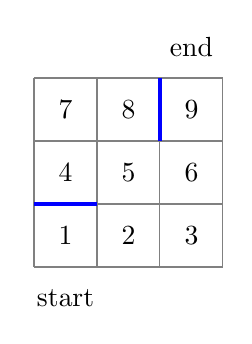
\begin{tikzpicture}[scale=0.8]
			\draw [thin,gray] (0,0) grid (3,3);
			\draw (0.5,0.5) node {1}
				  (1.5,0.5) node {2}
				  (2.5,0.5) node {3}
				  (0.5,1.5) node {4}
				  (1.5,1.5) node {5}
				  (2.5,1.5) node {6}
				  (0.5,2.5) node {7}
				  (1.5,2.5) node {8}
				  (2.5,2.5) node {9};
			\draw (0.5,-0.5) node {start}
				  (2.5,3.5) node {end};
			\draw [very thick,blue] (0,1) -- (1,1) (2,3) -- (2,2);
		\end{tikzpicture}
	\end{center}	
\end{column}
\end{columns}
\pause
Four trajectories beginning at $s_1$:
\begin{align*}
\tau_1 &:\quad 1,2,5,4,5,6,3,6,9 & R_{\tau_1} &= -8 \\
\tau_2 &:\quad 1,2,3,6,3,2,5,8,7,8,5,6,9 & R_{\tau_2} &= -12 \\
\tau_3 &:\quad 1,2,5,2,3,6,9 & R_{\tau_3} &= -6 \\
\tau_4 &:\quad 1,2,5,4,5,2,3,6,5,8,5,6,3,2,5,6,9 & R_{\tau_4} &= -16 \\
\end{align*}
\pause
\[ V(s_1) \approx \frac{R_{\tau_1} + R_{\tau_2} + R_{\tau_3} + R_{\tau_4}}{4} = \frac{(-8) + (-12) + (-6) + (-16)}{4} = -10.5 \]
	
\end{frame}


\begin{frame}{Re-using our trajectories to find $V(s_2)$}

\begin{columns}
\begin{column}{0.6\textwidth}
\begin{align*}
\tau_1 &:\quad 1,\red2,5,4,5,6,3,6,9 \\
\tau_2 &:\quad 1,\red2,3,6,3,\red2,5,8,7,8,5,6,9 \\
\tau_3 &:\quad 1,\red2,5,\red2,3,6,9 \\
\tau_4 &:\quad 1,\red2,5,4,5,\red2,3,6,5,8,5,6,3,\red2,5,6,9 \\
\end{align*}
\end{column}

\begin{column}{0.4\textwidth}
	\begin{center}
		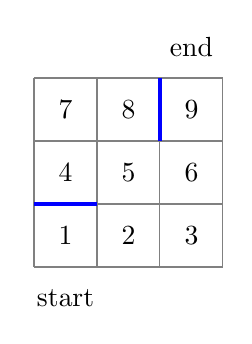
\begin{tikzpicture}[scale=0.8]
			\draw [thin,gray] (0,0) grid (3,3);
			\draw (0.5,0.5) node {1}
				  (1.5,0.5) node {2}
				  (2.5,0.5) node {3}
				  (0.5,1.5) node {4}
				  (1.5,1.5) node {5}
				  (2.5,1.5) node {6}
				  (0.5,2.5) node {7}
				  (1.5,2.5) node {8}
				  (2.5,2.5) node {9};
			\draw (0.5,-0.5) node {start}
				  (2.5,3.5) node {end};
			\draw [very thick,blue] (0,1) -- (1,1) (2,3) -- (2,2);
		\end{tikzpicture}
	\end{center}	
\end{column}
\end{columns}

\pskip
We can estimate $V(s_2)$ using the same trajectories because of the Markov Property. Every visit to $s_2$ is equivalent to new trajectory that begins at $s_2$.

\pskip
Some trajectories visit $s_2$ more than once. For example, $\tau_3$ has two returns $R=-5$ and $R=-3$.

\pskip
Every-visit average: $(-7 -11 -7 -5 -3 -15 -11 -3)/8=-7.75$. \\
Last-visit average: $(-7 -7 -3 -3)/4=-5$.

\end{frame}

\begin{frame}{Every-visit vs.\ last-visit}

\begin{itemize}
	\item Gridworld is deterministic and the agent has complete control over its actions.
	\item The agent should never visit the same state twice. Whatever sequence of actions are optimal after the second visit should have been selected after the first visit.
	\item For these problems, the last-visit estimate is closest to optimal.
\end{itemize}

\pskip
\begin{itemize}
	\item Stochastic problems can revisit the same state under the optimal policy.
	\item Imagine a stochastic airline, where planes fly to an unknown destination after takeoff.
	\begin{itemize}
		\item If you are trying to fly to Champaign, flights departing from O'Hare have the best chance of landing in Champaign.
		\item The optimal policy would be go back to O'Hare even if you've already been there.
	\end{itemize}
\end{itemize}

\end{frame}

\begin{frame}{Can we always find optimal policies from a value function?}

Yes. Acting \emph{greedy} with respect to a value function is optimal. Recall our definition of the value function
\[ V(s_i) = \mathbb{E}\{ r_i + r_{i+1} + \cdots + r_T \}. \]

\pskip
At any state $s_i$, the optimal policy follows the objective
\begin{align*} 
	 & \max_{a_i} \mathbb{E}\{ r_i + r_{i+1} + \cdots + r_T \} \\
	=& \max_{a_i} \mathbb{E}\{r_i\} + \mathbb{E}\{r_{i+1} + \cdots + r_T \} \\
	=& \max_{a_i} \mathbb{E}\{r_i\} + V(s_{i+1})
\end{align*}

\pause
For Gridworld, $r_i=-1$ for all states, so the optimal policy at state $s_i$ satisfies
\[ \max_{a_i} V(s_{i+1}) \]
i.e., select the action that brings the agent to the state with the largest value.

\end{frame}

\begin{frame}{Limitations of pure Monte Carlo}

\begin{columns}
\begin{column}{0.6\textwidth}
Random walks generate inefficient trajectories, as evidenced by the Monte Carlo value functions.

\bigskip
We can tell that some actions are bad even before we have a true value function.

\bigskip
Ideally, we would use early trajectories to speed up later trajectories.

\onslide<2->{
	\bigskip
	One solution is \textbf{generalized policy iteration}.
	\begin{enumerate}
		\item Use a random policy $\pi$ to generate trajectories and estimate $V(s)$.
		\item Adjust $\pi$ to be \emph{greedy} for $V(s)$.
		\item Repeat (1--2) until $\pi$ stops changing.
	\end{enumerate}
}
\end{column}

\begin{column}{0.4\textwidth}
	\begin{center}
		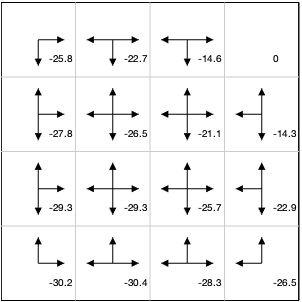
\includegraphics[width=\textwidth]{figures/gridworld1a.png}	

		\onslide<2->{
			\bigskip
			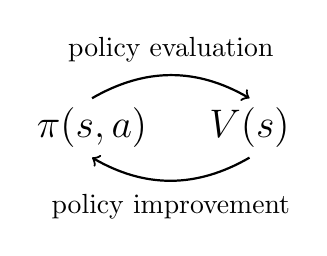
\begin{tikzpicture}
				\node (policy) at (-1,0) {\Large $\pi(s,a)$};
				\node (value) at (1,0) {\Large $V(s)$};
				\draw [thick] (policy.north) edge[bend left,->] (value.north);
				\draw [thick] (value.south) edge[bend left,->] (policy.south);
				\node at (0,1) {policy evaluation};
				\node at (0,-1) {policy improvement};
			\end{tikzpicture}
		}
	\end{center}
\end{column}
\end{columns}
	
\end{frame}

\begin{frame}{Does generalized policy iteration converge to an optimal policy?}

Yes, policy iteration is guaranteed to find optimal policies \emph{provided every state is visited an infinite number of times}.

\bigskip
In practice, policy iteration works well with finite visits, but \emph{tabular} methods require visiting every state. Without a visit, we have no way to tell if a policy should move to that state.

\pskip
For Gridworld, we started trajectories in every state to ensure a visit, but this was inefficient.

\pause
\begin{columns}
\begin{column}{0.5\textwidth}
For this board, why would we every visit the states in the upper left? 

\bigskip
No optimal policy would ever move ``up'' at the starting position.
\end{column}

\begin{column}{0.3\textwidth}
	\begin{center}
		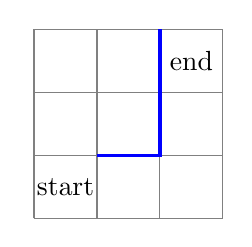
\begin{tikzpicture}[scale=0.8]
			\draw [thin,gray] (0,0) grid (3,3);
			\draw (0.5,0.5) node {start}
				  (2.5,2.5) node {end};
			\draw [very thick,blue] (1,1) -| (2,3);
		\end{tikzpicture}
	\end{center}	
\end{column}
\end{columns}

\pskip
Next time we'll learn \emph{online} methods to estimate a value function as we move through an MDP.
\end{frame}


\begin{frame}{Summary}

\begin{itemize}\lspace
	\item \textbf{Policy evaluation} computes $V(s)$ for a given policy.
	\item \textbf{Policy improvement} makes greedy improvements to a policy.
	\item If you don't have a good starting policy, behave randomly.
	\item Tabular methods track $V(s)$ for every state in the MDP. They require visiting every state many times and storing the results.
\end{itemize}

\end{frame}

\end{document}
